\section{Results}
\label{sec:results}
\begin{table}[t]
\centering\small
\caption{Mean score of the recommended policy over the \res{sites} test sites (\eur{}, three evaluation years each).}
\label{tab:means}
\begin{tabular}{lccc}
\toprule
Method & Full & Endpoint & Pre-experiment \\
\midrule
Prior-informed local BO (baseline) & \res{mean.baseline.full} & \res{mean.baseline.endpoint} & -- \\
GLM-5.3 Flash & \res{mean.glm.full} & \res{mean.glm.endpoint} & \res{mean.glm.initial} \\
MiMo V2.6 Flash & \res{mean.mimo.full} & \res{mean.mimo.endpoint} & \res{mean.mimo.initial} \\
DeepSeek V4.1 Flash & \res{mean.deepseek.full} & \res{mean.deepseek.endpoint} & \res{mean.deepseek.initial} \\
Fixed reference (no experiments) & \multicolumn{3}{c}{\res{mean.fixed.reference}} \\
\bottomrule
\end{tabular}
\end{table}

\begin{figure}[t]
\centering
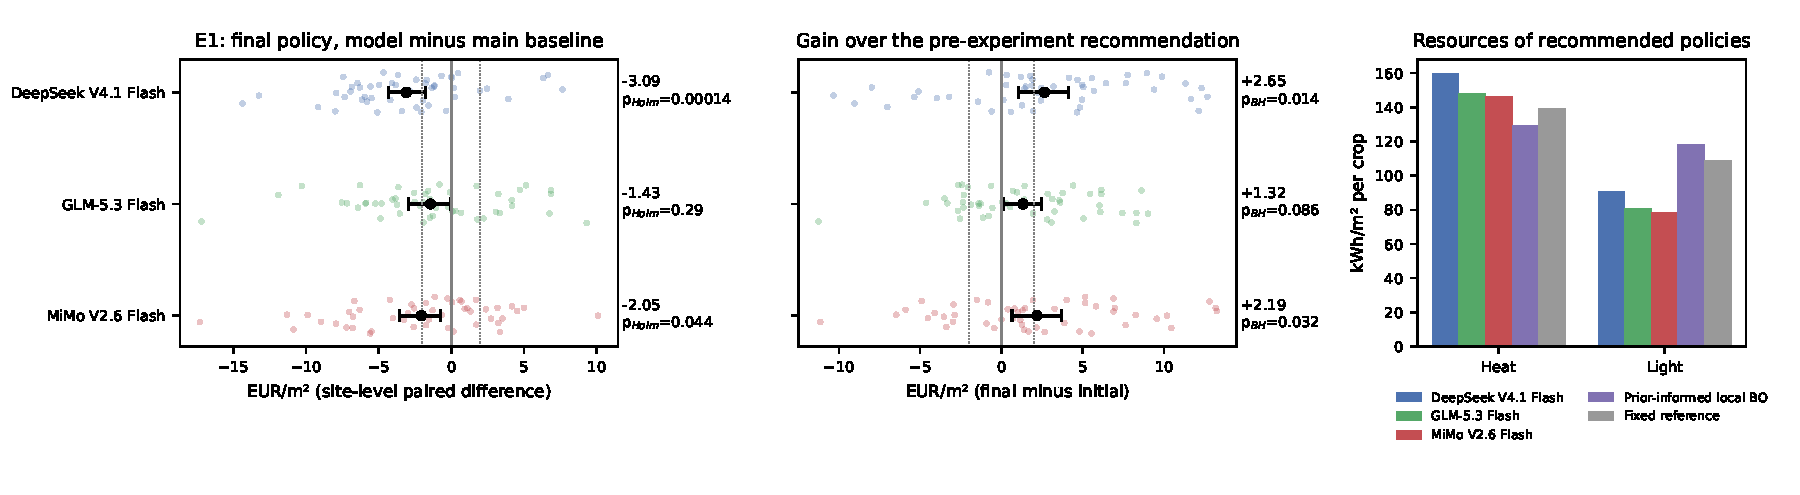
\includegraphics[width=\linewidth]{figures/fig2_e1.pdf}
\caption{Language models end near the grower setting, well below the baseline. Left: site-level paired difference between each model's final (Full) policy and the baseline's; dots are sites, bars BCa 95\% intervals, dotted lines the smallest effect of interest ($\pm2$~\eur{}); p-values Holm-adjusted. Middle: gain over the model's own pre-experiment recommendation (BH-adjusted). Right: heat and light per crop of the recommended policies in the evaluation runs.}
\label{fig:e1}
\end{figure}

\subsection{Language models end near the grower setting, well below a domain-informed optimiser (RQ1, E1)}
\label{sec:rq1}
All three models ended clearly below the baseline (Figure~\ref{fig:e1}, Table~\ref{tab:means}): DeepSeek by \res{E1.deepseek.mean}~\eur{} [\res{E1.deepseek.lo}, \res{E1.deepseek.hi}], MiMo by \res{E1.mimo.mean} [\res{E1.mimo.lo}, \res{E1.mimo.hi}] and GLM by \res{E1.glm.mean} [\res{E1.glm.lo}, \res{E1.glm.hi}], each with $p_\text{Holm}$ \res{E1.glm.p}; every interval lies beyond the smallest effect of interest. The models did end better than they started, by \res{learn.deepseek.mean} (DeepSeek, $p_\text{BH}$ = \res{learn.deepseek.p}), \res{learn.mimo.mean} (MiMo, \res{learn.mimo.p}) and \res{learn.glm.mean}~\eur{} (GLM, \res{learn.glm.p}), significantly only for DeepSeek, and stopped near the fixed reference (\res{vsfixed.glm.mean}, \res{vsfixed.mimo.mean} and \res{vsfixed.deepseek.mean}~\eur{}), which the baseline exceeded by \res{vsfixed.baseline.mean} [\res{vsfixed.baseline.lo}, \res{vsfixed.baseline.hi}].

The gap has two parts. The first is the starting point: the baseline starts from the fixed reference (\res{mean.fixed.reference}~\eur{}), which the models are not given, while their own pre-experiment recommendations scored \res{range.initial.lo}--\res{range.initial.hi}. The second is the search itself: within the year the baseline gained \res{vsfixed.baseline.mean}~\eur{} over its starting point and the models \res{range.learn.lo} to \res{range.learn.hi} over theirs. The two kinds of policy also differ in style: the models' final policies used less supplemental light than the baseline's (\res{range.llm.full.light.lo}--\res{range.llm.full.light.hi} against \res{res.baseline.full.light}~kWh/m$^2$ per crop) and more heat (\res{range.llm.full.heat.lo}--\res{range.llm.full.heat.hi} against \res{res.baseline.full.heat}).

\begin{figure}[t]
\centering
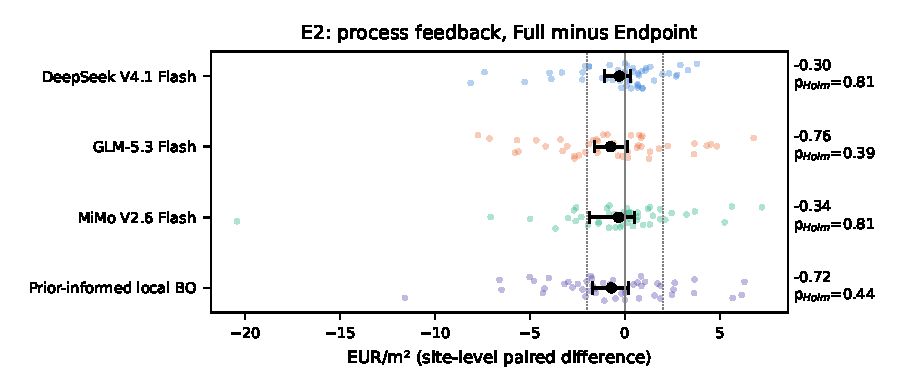
\includegraphics[width=0.75\linewidth]{figures/fig3_e2.pdf}
\caption{No method profits from in-season process feedback: site-level paired difference between the Full and Endpoint branches of each method (Holm-adjusted).}
\label{fig:e2}
\end{figure}

\subsection{No method profits from in-season process feedback (RQ2, E2)}
\label{sec:rq2}
Being able to read process measurements during the season did not improve the final policy of any method (Figure~\ref{fig:e2}). Full minus Endpoint was \res{E2.deepseek.mean} [\res{E2.deepseek.lo}, \res{E2.deepseek.hi}] for DeepSeek, \res{E2.glm.mean} [\res{E2.glm.lo}, \res{E2.glm.hi}] for GLM, \res{E2.mimo.mean} [\res{E2.mimo.lo}, \res{E2.mimo.hi}] for MiMo and \res{E2.baseline.mean} [\res{E2.baseline.lo}, \res{E2.baseline.hi}]~\eur{} for the baseline; none is significant, every upper bound lies well below the 2~\eur{} effect of interest, and the feedback gains did not differ between methods (all $p_\text{BH}\ge$ \res{range.gaindiff.p.lo}).

The campaign records show why: the models ran the facility as two synchronous batches. In \res{range.fb.waitpct.lo}--\res{range.fb.waitpct.hi}\% of their Full branches the first new crop was planted only after the first wave had closed and released its totals, so in-season readings could not change what was planted next (Appendix Figure~\ref{fig:timelines}). Before that planting the Full branches read a sensor channel only \res{range.fb.reads.lo}--\res{range.fb.reads.hi} times on average and called the process predictor \res{range.fb.predictor.lo}--\res{range.fb.predictor.hi} times. A running crop was stopped in a single campaign (a GLM Full branch, \res{fb.glm.stops} of \res{fb.glm.campaigns}), and the Full and Endpoint branches planted their later crops in the same compartments on the same days in \res{fb.deepseek.sameschedule}, \res{fb.glm.sameschedule} and \res{fb.mimo.sameschedule} of \res{fb.deepseek.campaigns} campaigns (DeepSeek, GLM, MiMo). The models' stated reasons on test site 0 (repeat 0, the rule used for Figure~\ref{fig:teaser}) are typical: \emph{``Let the baseline crops finish their 180-day cycle so totals are released''} (DeepSeek, day 150) and, after consulting the process predictor at day 30, \emph{``Let the four batch-1 crops run to maturity; results will release at closure\ldots''} (GLM). The baseline, which by construction staggers two compartments at mid-season with the process predictor, did not gain from the feedback either, which suggests that the in-season signal available through the predictor added little in this task.

\begin{figure}[t]
\centering
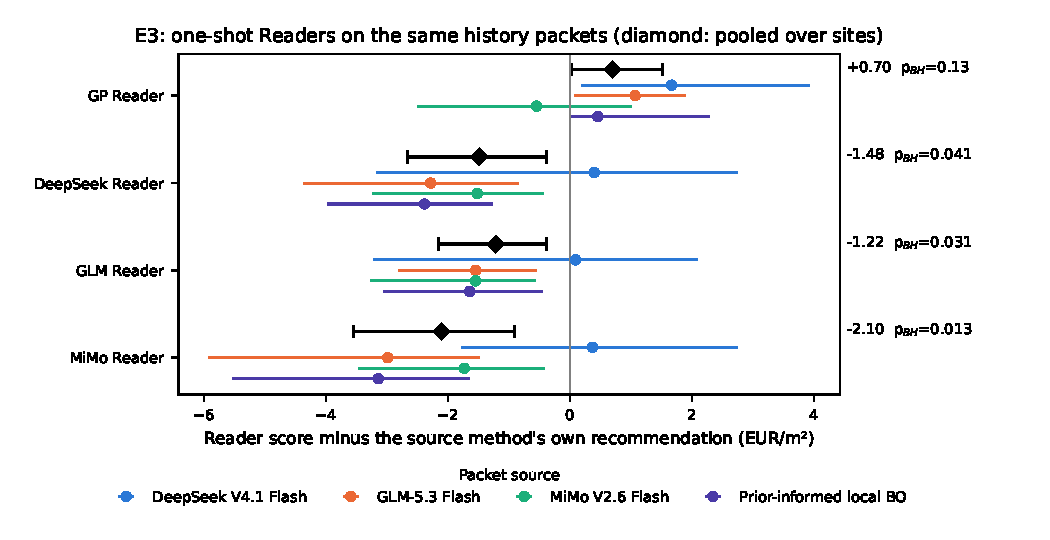
\includegraphics[width=0.85\linewidth]{figures/fig4_e3.pdf}
\caption{Reading the final evidence is not the bottleneck. Reader swap gain: each Reader's recommendation from a history packet minus the recommendation of the method that collected the packet, by packet source (16 packets each, BCa 95\% intervals) and pooled over sites (diamonds; BH-adjusted over the joint secondary family).}
\label{fig:e3}
\end{figure}

\subsection{Reading the final evidence is not the bottleneck (RQ3, E3)}
\label{sec:rq3}
With a committed seed we drew 64 history packets from repeat-0 Full campaigns, 16 per method on distinct sites; a packet holds the public evidence the method had before recommending and names no method. Each was read by the GP Reader (the baseline's own recommendation step) and by each model in one shot. The \emph{Reader swap gain} is the Reader's recommendation score minus the source method's own on the same packet (BH over the joint secondary family of \res{secondary.family} tests).

No Reader's pooled swap gain differed significantly from zero (Figure~\ref{fig:e3}): \res{E3.deepseek.mean}~\eur{} [\res{E3.deepseek.lo}, \res{E3.deepseek.hi}] for DeepSeek ($p_\text{BH}$ = \res{E3.deepseek.p}), \res{E3.glm.mean} [\res{E3.glm.lo}, \res{E3.glm.hi}] for GLM (\res{E3.glm.p}), \res{E3.mimo.mean} [\res{E3.mimo.lo}, \res{E3.mimo.hi}] for MiMo (\res{E3.mimo.p}) and \res{E3.gp.mean} [\res{E3.gp.lo}, \res{E3.gp.hi}] for the GP Reader (\res{E3.gp.p}). Every pooled interval lies within the 2~\eur{} effect of interest and well short of the E1 gap. Even the baseline's numerical Reader, given a model's evidence, gained on average at most \res{range.E3.gp.llm.hi}~\eur{} on any model's packets, a small fraction of the E1 gap. Reading the same evidence better would therefore close little of the gap, which points upstream of reading: to where the models start and which policies they try. As a consistency check, the GP Reader returned exactly the baseline's final policy on all 16 baseline packets. By source the picture is mixed and, with 16 packets per cell, descriptive only; because each source's packets come from different sites, E3 cannot compare the quality of evidence across methods directly.

\subsection{Where the conclusions hold}
\label{sec:robust}
\paragraph{Headroom.} On \res{ref.sites} random test sites, a numerical search for the best feasible policy found policies that beat the fixed reference by \res{ref.headroom}~\eur{} on average; two repeated searches differed by \res{ref.err.lo} and \res{ref.err.hi}~\eur{}, so the best-known values are lower bounds with that error. On these sites the baseline's final policies were \res{ref.baseline.vsfixed} relative to the fixed reference, most of the estimated headroom, while the models' were \res{ref.glm.vsfixed} (GLM), \res{ref.mimo.vsfixed} (MiMo) and \res{ref.deepseek.vsfixed} (DeepSeek).

\paragraph{Sensitivity.} The size of the E1 gap depends on two environment assumptions. With the side-wall heat exchange set to 4~W/m$^2$K instead of each site's drawn value (1--3) on \res{ueff.sites} random sites, the model-minus-baseline differences shrank to \res{ueff.4.deepseek} (DeepSeek), \res{ueff.4.glm} (GLM) and \res{ueff.4.mimo}~\eur{} (MiMo), against \res{ueff.main.deepseek}, \res{ueff.main.glm} and \res{ueff.main.mimo} on the same sites at the drawn value; the method ranking \res{ueff.4.rankchange} at 4~W/m$^2$K and was \res{ueff.0.rankchange} at 0. The models' policies use less light and more heat than the baseline's, and a larger exchange with the warmer neighbouring spaces favours them. With a fruit dry-matter fraction of \setting{0.07} instead of \setting{0.06} the E1 differences shrank to \res{dm.0.07.deepseek} (DeepSeek), \res{dm.0.07.glm} (GLM) and \res{dm.0.07.mimo} (MiMo); at \setting{0.05} they grew to \res{dm.0.05.deepseek}, \res{dm.0.05.glm} and \res{dm.0.05.mimo}. The sign of E1 held in every setting except MiMo at the highest heat exchange, and E2 was insensitive to the dry-matter fraction.

\paragraph{Cost and failure modes.} A branched campaign cost on average USD \res{cost.deepseek} (DeepSeek, \res{calls.deepseek} calls), \res{cost.glm} (GLM, \res{calls.glm}) and \res{cost.mimo} (MiMo, \res{calls.mimo}). MiMo produced markedly more format errors (\res{formaterr.mimo} per Full branch against \res{formaterr.deepseek} and \res{formaterr.glm}); these are part of the method's result.
